\subsection{Decorator}

\textbf{Scopo}: Strutturale \\
\textbf{Raggio d'azione}: Oggetti

\paragraph{Definizione} Il pattern decorator permetter di aggiungere dinamicamente responsabilità ad un oggetto. Fornisce un'alternativa flessibile all'uso dell'ereditarietà come strumento per l'estensione delle funzionalità.

\paragraph{Problema} Talvolta è necessario aggiungere responsabilità ad un singolo oggetto e non ad un intera classe.

Esempio: Libreria per la realizzazione di interfacce utente deve permettere di aggiungere bordi o altri elementi a ciascun componente grafico.

Ricorrere all'ereditarietà complicherebbe la cosa, andrebbero create sottoclassi per ogni componente aggiuntivo, in più renderebbe difficile comporre più estensioni di comportamento.

\paragraph{Soluzione} Racchiudere il componente da decorare dentro un altro che sarà responsabile di disegnare il bordo o aggiungere altri componenti visivi. L'oggetto contenitore è detto \textit{decoratore} ed ha la stessa interfaccia dell'oggetto decorato così da poter essere trasparente al client. È possibile che svolga azioni aggiuntive prima o dopo aver trasferito la richiesta all'oggetto decorato.

\begin{figure}[H]
    \centering
    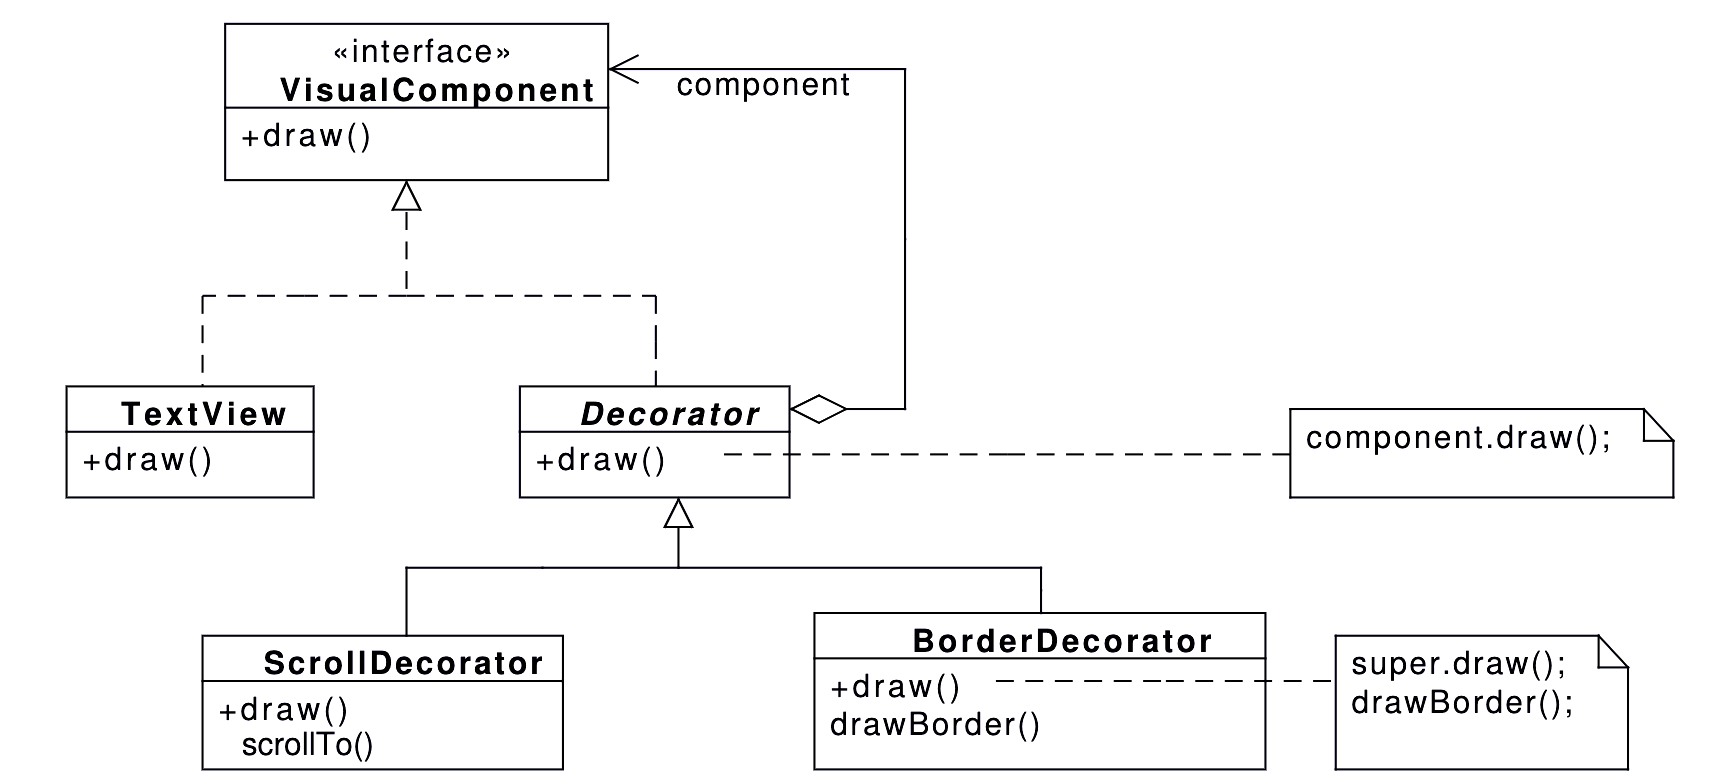
\includegraphics[width=1\linewidth]{assets/pattern/decorator/decorator-esempio.png}
    \caption{Esempio di utilizzo del pattern}
\end{figure}

Nell'esempio l'interfaccia VisualComponent definisce il tipo generico di componenti visuali. La classe TextView consente di visualizzare del testo in una finestra. La classe astratta Decorator inoltra semplicemente le richieste al componente incapsulato. BorderDecorator e ScrollDecorator consentono rispettivamente di aggiungere bordi e barre di scorrimento.

\paragraph{Struttura e Conseguenze} Il pattern è composto dai seguenti partecipanti:
\begin{itemize}
    \item \textbf{ServiceIF} (VisualComponent): definisce l'interfaccia comune per gli oggetti ai quali possono essere aggiunte nuove responsabilità dinamicamente.
    \item \textbf{ConcreteService} (TextView): definisce un oggetto al quale possono essere aggiunte ulteriori responsabilità
    \item \textbf{Decorator}: mantiene un riferimento ad un oggetto di tipo ServiceIF e, al contempo implementa l'interfaccia ServiceIF.
    \item \textbf{ConcreteDecorator} (ScrollDecorator, BorderDecorator): aggiunge responsabilità al componente
\end{itemize}


\begin{figure}[H]
    \centering
    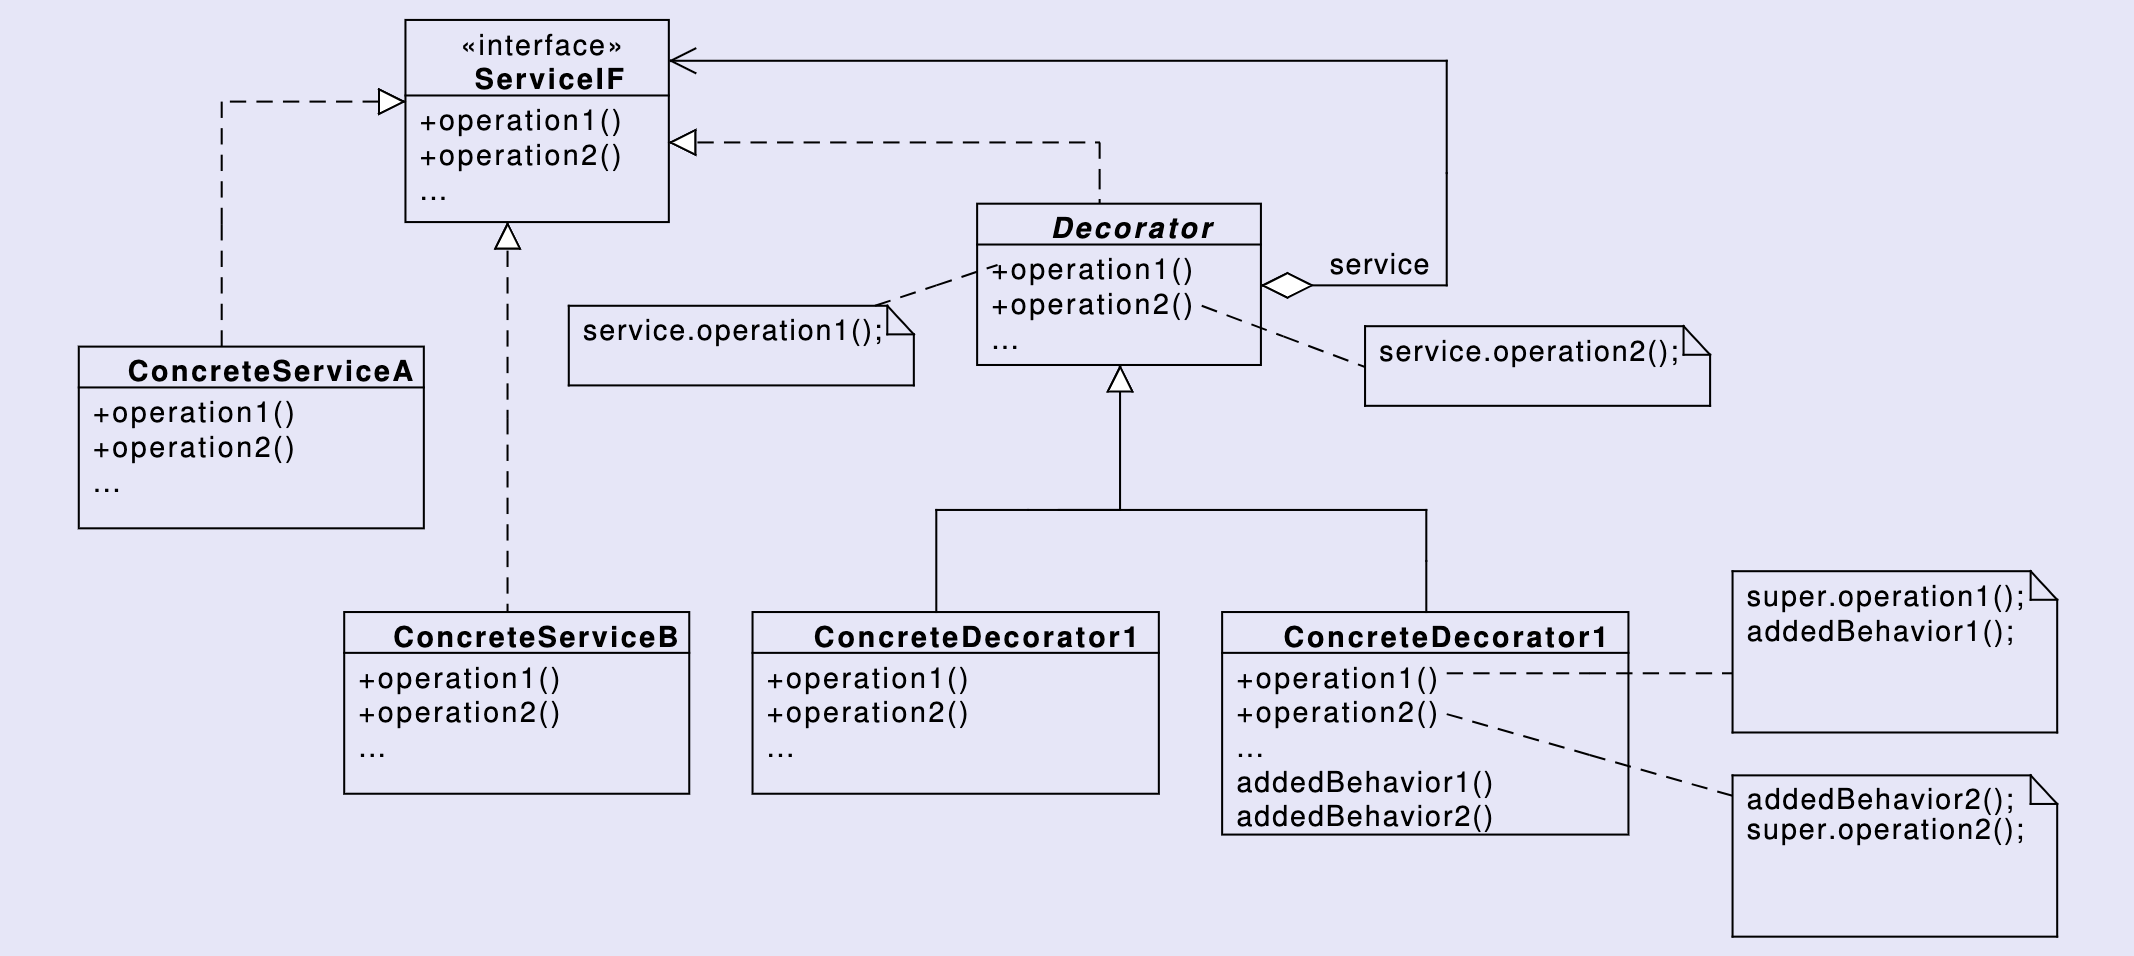
\includegraphics[width=1\linewidth]{assets/pattern/decorator/decorator-struttura.png}
    \caption{Struttura del pattern Decorator}
\end{figure}

\begin{figure}[H]
    \centering
    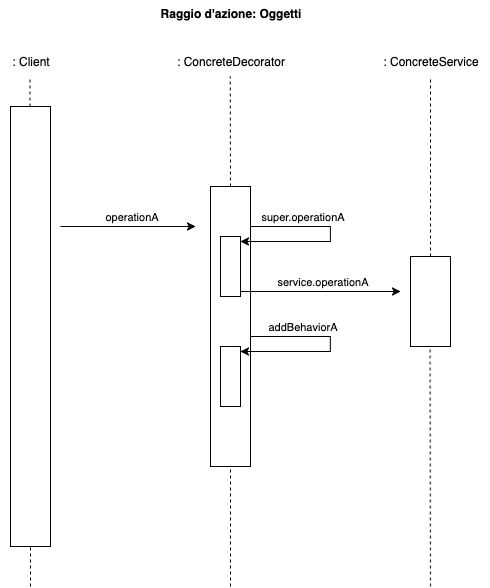
\includegraphics[width=1\linewidth]{assets/pattern/decorator/decorator-activity.drawio.png}
    \caption{Activity diagram del pattern Decorator}
\end{figure}


\newpage